\documentclass[12pt]{article}
\usepackage[a4paper, total={6in, 10in}]{geometry}
\usepackage{graphicx}
\graphicspath{{figs/}} 



\title{Title} 
\author{Surname Forename}
\date{\today}

\begin{document}
\maketitle
\thispagestyle{empty} %No number



\begin{abstract}
This is the paper's abstract \ldots
\end{abstract}

\section{Introduction}
This is time for all good men to come to the aid of their party!

\paragraph{Outline}
The remainder of this article is organized as follows.
Section~\ref{previous work} gives account of previous work.
Our new and exciting results are described in Section~\ref{results}.
Finally, Section~\ref{conclusions} gives the conclusions.


\section{Figues}
Figure \ref{fig:cacaxtla} illustrate the rules of Cacaxtla.

%%---------------------------------(FIGURE)-------------------------------------
\begin{figure}[!h]
\centering
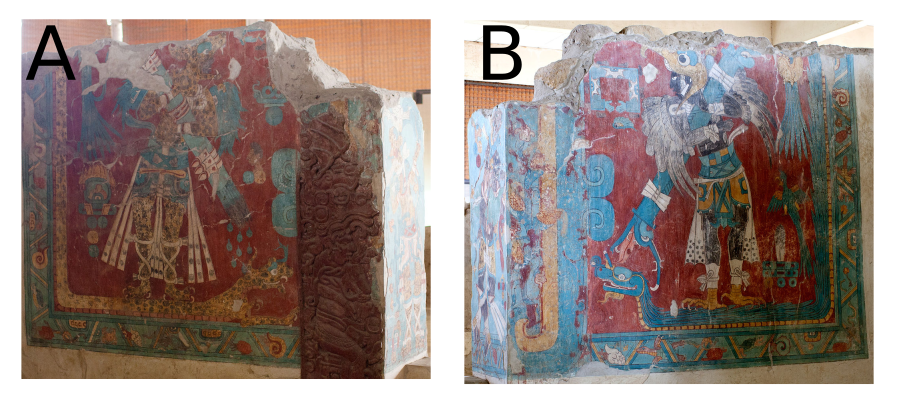
\includegraphics[width=1.0\textwidth]{cacaxtlarulers}
    \caption{
	{\bf Rulers of Cacaxtla.}
	 (A) Feline man and (B) bird man.
	The bird man is associated with Quetzalcoatl, 
	the generous deity who taught people the arts and agriculture. 
	The feline man is associated with the rains that fertilize the earth \cite{wiki:cacaxtla}.
        }
\label{fig:cacaxtla}
\end{figure}
%%---------------------------------(FIGURE)------------------------------------




\section{Previous work}\label{previous work}
A much longer \LaTeXe{} example was written by Gil~\cite{Gil:02}.

\section{Results}\label{results}
In this section we describe the results.

\section{Conclusions}\label{conclusions}
We worked hard, and achieved very little.

\bibliographystyle{apalike}
\bibliography{references}




\end{document}
